\pagebreak

\section{Modèle de Porter}

\begin{figure}[H]
	\begin{center}
		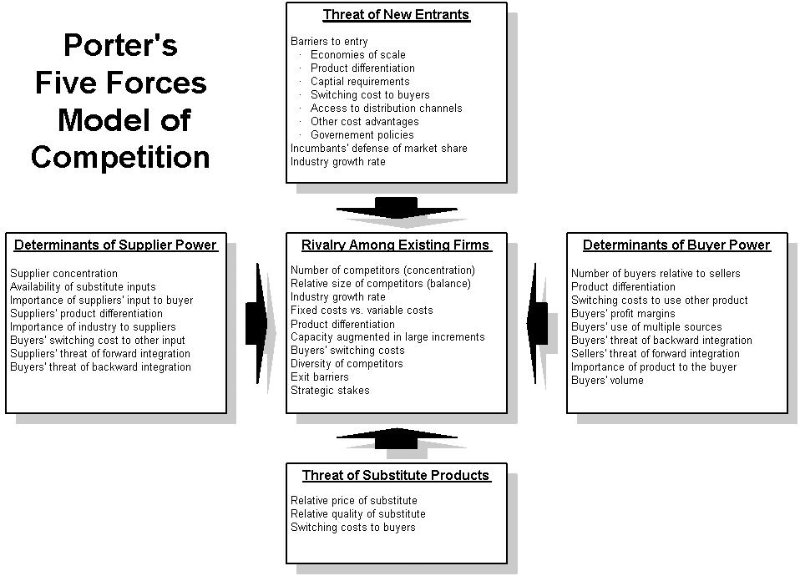
\includegraphics[scale=0.48]{images/porter/porter_1}
		\caption{Modèle de Porter}
		\label{inclusion}
	\end{center}
\end{figure}

\section{Analyse de marché}

\subsection{Définition du marché}

Cette étude porte sur les sociétés de Fret Aérien Civil Traditionnelles (FACT) qui gèrent leur propre flotte aérienne pour le transport de biens. Ce qui exclus le fret militaire ainsi que les logisticiens, entreprises de fret "virtuelles", qui font du point à point et louent des charters ou achètent des emplacements aux compagnies de fret traditionnlles. Les compagnies virtuelles constituent donc à la fois des clients pour le Fret Aérien Civil Traditionnel (FACT) qui permet à ces dernières d'optimiser le remplissage de leurs avions-cargo, mais aussi une forme de concurrence puisque le fret transporté au nom du logisticien est "perdu" pour tous les transporteurs classiques, y compris celui qui assure réellement le service. 

\subsection{Description des produits concernés}
Pour évaluer la concurrence, il convient d'étudier en premier lieu, le type de produits transportés. En effet, le pétrole ou le gaz, ne sont pas en général, transportés par avions ; sur ces matières premières, il n'existe donc pas de concurrence maritime, fluviale, routière ou par oléoduc/gazoduc. 

Le fret aérien concerne donc :

\begin{itemize}
	\item Produits à valeur ajoutée : ....
	\item Produits périssables : fleurs, fruits, 
	\item Animaux,
	\item Produits urgents ou à finalités humanitaires.
\end{itemize}



\subsection{Bla2}





\subsection{Bla3}

